Beschreiben Sie den Viertel des Einheitskreises im ersten Quadranten
als eine Bézier-Kurve mit Kontrollpunkten 
\[
(1,0),\quad (1,a), \quad (a,1) \quad\text{und}\quad (0,1).
\]
Wählen Sie $a$ so, dass die Bézier-Kurve durch den Punkt
$(1/\sqrt{2},1/\sqrt{2})$ verläuft.
\begin{teilaufgaben}
\item
Bestimmen Sie die maximale Abweichung der Bézier-Kurve vom Einheitskreis.
\item
Vergleichen Sie die Approximation durch die Bézier-Kurve mit
der Parametrisierung $t\mapsto (\cos\frac{\pi}2t,\sin\frac{\pi}2t)$ des
Einheitskreises.
\end{teilaufgaben}
\begin{figure}
\centering
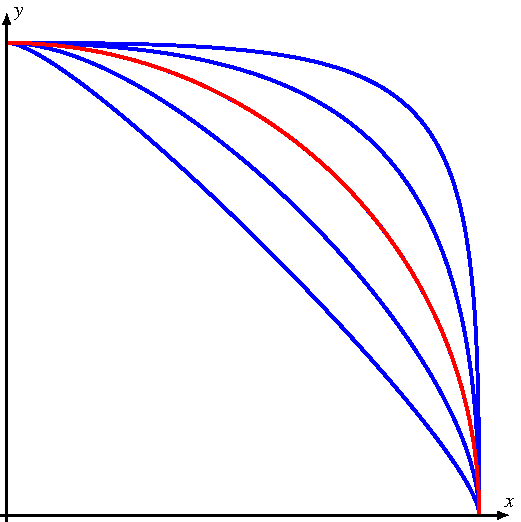
\includegraphics{chapters/30-interpolation/uebungsaufgaben/3003kreis.pdf}
\caption{Approximation eines Kreises (hellrote Fläche) mit Hilfe einer
Bézier-Kurve durch die Punkt $(1,0)$, $(1,a)$, $(a,1)$ und $(0,1)$ (rote
Punkte).
Für $a=\frac43(\!\sqrt{2}-1)$ verläuft die Bézier-Kurve durch den 
Punkt $(\sqrt{2}/2,\sqrt{2}/2)$ auf dem Einheitskreis.
\label{3003:figure:kreis}}
\end{figure}

\begin{loesung}
Die Bézier-Kurve hat die Koordinaten
\begin{align*}
x(t)
&=
(1-t)^3\cdot1
+
3(1-t)^2t\cdot1
+
3(1-t)t^2\cdot a
+
t^3\cdot 0,
\\
y(t)
&=
(1-t)^3\cdot0
+
3(1-t)^2t\cdot a
+
3(1-t)t^2\cdot 1
+
t^3\cdot 1.
\end{align*}
Aus Symmetriegründen schneidet die Bézier-Kurve die $45^\circ$-Gerade
im Parameter-Wert $t=\frac12$, also
\[
x({\textstyle\frac12})
=
\frac18(1+3+3a+0)
=
\frac{3a+4}8
\qquad
y({\textstyle\frac12})
=
\frac18(0+3a+3+1).
\]
Daraus ergibt sich 
\[
3a+4=4\sqrt{2}
\qquad\Rightarrow\qquad
a = \frac43(\sqrt{2}-1)
\approx
0.5522847.
\]
\begin{figure}
\centering
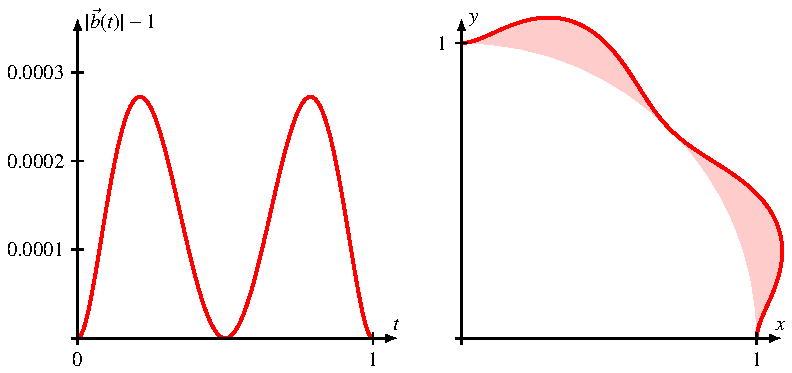
\includegraphics{chapters/30-interpolation/uebungsaufgaben/radiusfehler.pdf}
\caption{Radiusfehler $|\vec{b}(t)|-1$ der Bézier-Approximation $\vec{b}(t)$
des Einheitskreises.
Der Fehler des Radius (links) ist sehr gering, rechts ist die Abweichung
vom Kreis 500-fach überhöht dargestellt.
\label{3003:figure:radiusfehler}}
\end{figure}
\begin{figure}
\centering
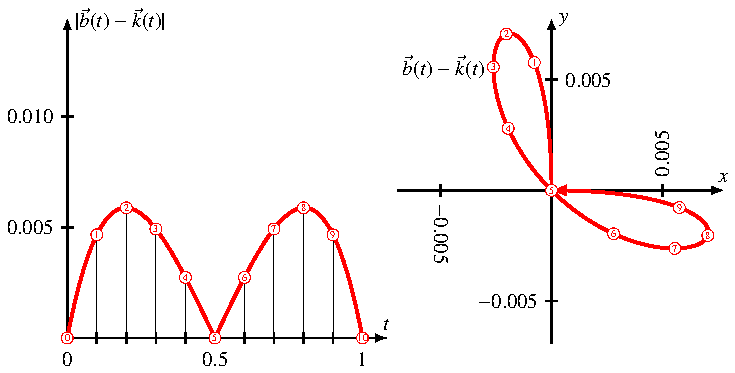
\includegraphics{chapters/30-interpolation/uebungsaufgaben/abweichungen.pdf}
\caption{Fehler der Bézier-Approximation $\vec{b}(t)$ des Einheitskreises,
der üblicherweise mit $\vec{k}(t)=(\cos t\frac{\pi}2,\sin t\frac{\pi}2)$
parametrisiert wird.
Die Abweichung $\vec{b}(t)-\vec{k}(t)$ ist etwa 30 mal grösser als
$|\vec{b}(t)|-1$, aber immer noch sehr klein.
Rechts ist der Differenz-Vektor $\vec{b}(t)-\vec{k}(t)$ dargestellt.
\label{3003:figure:abweichungen}}
\end{figure}
Damit kann man jetzt die Fehlerbetrachtungen der beiden Teilaufgaben
durchführen:
\begin{teilaufgaben}
\item
Abbildung~\ref{3003:figure:radiusfehler} zeigt den Fehler des
Radius $|\vec{b}(t)|-1$.
Die Bézier-Kurve verläuft immer ausserhalb des Kreises.
In Abbildung~\ref{3003:figure:radiusfehler} rechts ist der Radiusfehler
500-fach überhöht dargestellt.
\item
Der Geschwindigkeitsvektor der Bézier-Kurve zur Zeit $t=0$ ist nach
Satz~\ref{buch:bezier:satz} das dreifache des Vektors zwischen den ersten
zwei Punkten, also
\[
\dot{\vec{b}}(0)
=
\begin{pmatrix}
\dot{x}(0)\\
\dot{y}(0)\\
\end{pmatrix}
=
\begin{pmatrix}
0\\
3a
\end{pmatrix}
=
\begin{pmatrix}
0
\\
4(\sqrt{2}-1)
\end{pmatrix}
\approx
\begin{pmatrix}
0
\\
1.65685
\end{pmatrix}.
\]
Der Geschwindigkeitsvektor der Kreisparametrisierung $\vec{k}(t)$ ist
dagegen
\[
\dot{\vec{k}}(0)
=
\begin{pmatrix}
0\\\frac\pi2
\end{pmatrix}
\approx
\begin{pmatrix}
0\\
1.57079
\end{pmatrix}.
\]
Der Punkt auf der Bézier-Kurve entfernt sich daher zu Beginn mit der
Geschwindigkeit
\[
\vec{v}(0)
=
\dot{\vec{b}}(0) - \dot{\vec{k}}(0)
\approx
\begin{pmatrix}
0
\\
0.0860579
\end{pmatrix}
\]
vom Punk $\vec{k}(t)$.
Die graphische Darstellung in Abbildung~\ref{3003:figure:abweichungen}
zeigt, dass ungefähr zur Zeit $t=0.2$ die grösste Entfernun eintritt.
Der Unterschied kann also nicht grösser sein als
$0.2\cdot 0.0860579\approx 0.017$, was immer noch erstaunlich gut ist.
\qedhere
\end{teilaufgaben}
\end{loesung}
